\section{Definizioni}
\begin{itemize}
    \item Un albero binario ha la caratteristica che ogni vertice può avere al massimo 2 figli.
        \begin{figure}[H]
        \centering
        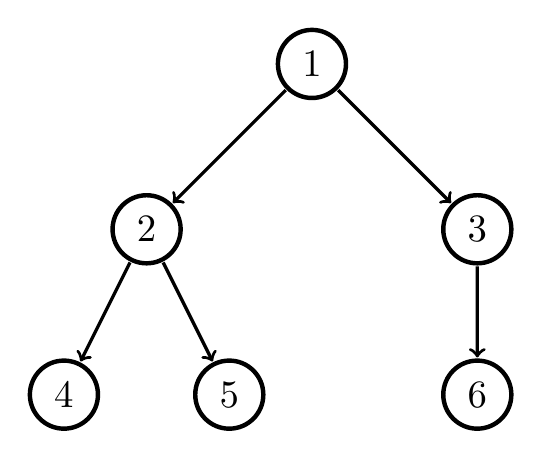
\begin{tikzpicture}[
            scale=1.4, 
            every node/.style={draw, circle, ultra thick, scale=1.4}, 
            edge from parent/.style={draw, very thick},
            level 1/.style={sibling distance=30mm},
            level 2/.style={sibling distance=15mm},
            ->
            ]
        \node{1}
            child { node{2}
                child { node{4} }
                child { node{5} }
            }
            child { node{3}
                child { node{6} }
            };
        \end{tikzpicture}
        \caption{Esempio di albero binario.}
        \label{fig:example_binary_tree}
        \end{figure}
    \item Un albero binario pieno ha $0$ o $2$ figli a ogni vertice.
        \begin{figure}[H]
        \centering
        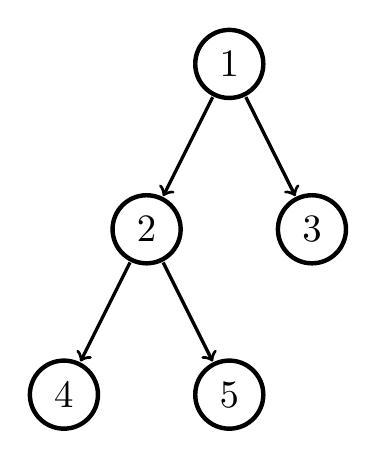
\begin{tikzpicture}[
            scale=1.4, 
            every node/.style={draw, circle, ultra thick, scale=1.4}, 
            edge from parent/.style={draw, very thick},
            ->
            ]
        \node{1}
            child { node{2}
                child { node{4} }
                child { node{5} }
            }
            child { node{3}
            };
        \end{tikzpicture}
        \caption{Esempio di albero binario pieno.}
        \label{fig:example_full_binary_tree}
        \end{figure}
    \item Un albero binario pieno completo ha $2$ figli a ogni vertice.
        \begin{figure}[H]
        \centering
        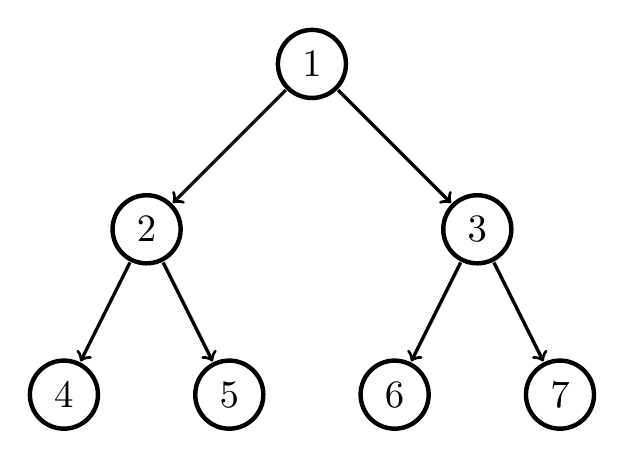
\begin{tikzpicture}[
            scale=1.4, 
            every node/.style={draw, circle, ultra thick, scale=1.4}, 
            edge from parent/.style={draw, very thick},
            level 1/.style={sibling distance=30mm},
            level 2/.style={sibling distance=15mm},
            ->
            ]
        \node{1}
            child { node{2}
                child { node{4} }
                child { node{5} }
            }
            child { node{3}
                child { node{6} }
                child { node{7} }
            };
        \end{tikzpicture}
        \caption{Esempio di albero binario pieno completo.}
        \label{fig:example_complete_full_binary_tree}
        \end{figure}
    \item Poiché vi è un limite sui figli che ogni vertice può avere, ad ogni profondità/livello $d$ dell'albero ci possono essere al massimo $2^d$ vertici.
\end{itemize}

\section{Definizione ricorsiva albero binario pieno}
\textbf{Passo base}: $T=(\{r\}, \emptyset)$ è un albero binario pieno.

\textbf{Passo ricorsivo}: Supponiamo che $T_1(V_1, E_1)$ e $T_2(V_2, E_2)$ siano alberi binari pieni  disgiunti, cioè $V_1 \cap V_2 = \emptyset$ con radici $r_1 \in V_1$ e $r_2 \in V_2$. 
Allora $T=(V, E)$ si ottiene ponendo come radice un nodo $r \not\in V_1 \cup V_2$ e da $r$ si aggiunge un arco a $r_1 \in V_1$ e $r_2 \in V_2$.

$V = \{r\} \cup V_1 \cup V_2$

$E = \{(r, r_1), (r, r_2)\} \cup E_1 \cup E_2$ \\
$T = (V, E)$ è un albero binario pieno.

\section{Definizione ricorsiva di albero binario}
\textbf{Passo base}: $T=(\emptyset, \emptyset)$ è un albero binario.

\textbf{Passo ricorsivo} Supponiamo che $T_1(V_1, E_1)$ e $T_2(V_2, E_2)$ siano alberi binari disgiunti, cioè $V_1 \cap V_2 = \emptyset$ con radici $r_1 \in V_1$ e $r_2 \in V_2$.
Allora $T=(V, E)$ si ottiene ponendo come radice un nodo $r \not\in V_1 \cup V_2$ e da $r$ si aggiunge un arco a $r_1 \in V_1$ e $r_2 \in V_2$.

$V = \{r\} \cup V_1 \cup V_2$

$E = \{(r, r_1), (r, r_2)\} \cup E_1 \cup E_2$ \\
$T = (V, E)$ è un albero binario.
